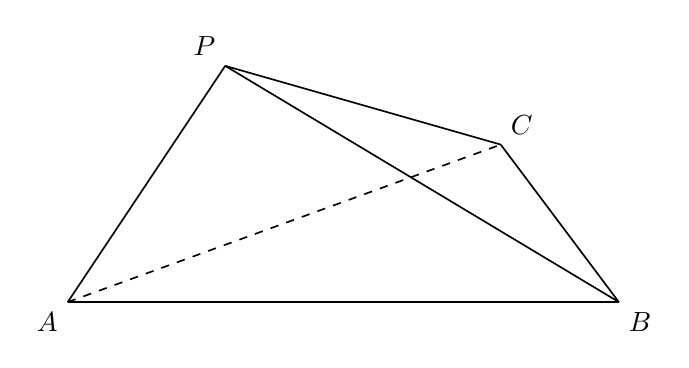
\begin{tikzpicture}[x=1cm,y=1cm,font=\normalsize,line width=.6pt]
\coordinate (A) at (0,0);
\coordinate (B) at (7,0);
\coordinate (P) at (2,3);
\coordinate (C) at (5.5,2);
\draw (A) -- (B);
\draw (A) -- (P);
\draw (P) -- (B);
\draw (P) -- (C);
\draw (C) -- (B);
\draw[dashed] (A) -- (C);
\node[below left] at (A) {$A$};
\node[below right] at (B) {$B$};
\node[above left] at (P) {$P$};
\node[above right] at (C) {$C$};
\end{tikzpicture}
